% !TEX root = ./notes_template.tex
\documentclass[11pt,twoside]{book}
\usepackage[mono=false]{libertine} % new linux font, ignore mono

% avoid bugs with xy-pic, luatex, pdftex version
% \input{luatex-pdf}
\usepackage{luatex85}
% \usepackage[all]{xy}

%\renewcommand{\baselinestretch}{1.05}
\usepackage{amsmath,amsthm,amssymb,mathrsfs,amsfonts,dsfont}
\usepackage[spanish]{babel}
\usepackage{epsfig,graphicx}
\usepackage{tabularx}
\usepackage{blkarray}
\usepackage{slashed}
\usepackage{color}
\usepackage{listings}
\usepackage{caption}
% \usepackage{fullpage}
\usepackage{lipsum} % provides dummy text for testing
\usepackage[toc,title,titletoc,header]{appendix}
\usepackage{minitoc}
\usepackage{color}
\usepackage{multicol} % two-col ToC
\usepackage{bm}
\usepackage{imakeidx} % before hyperref
\usepackage{hyperref}
\hypersetup{
    colorlinks=true,
    citecolor=magenta,
    linkcolor=blue,
    filecolor=green,      
    urlcolor=cyan,
    % hypertexnames=false,
}
\usepackage[capitalise]{cleveref}
\usepackage{subcaption}
\usepackage{enumitem}
\usepackage{mathtools}
\usepackage{physics}
\usepackage[linesnumbered,ruled,vlined,algosection]{algorithm2e}
\SetCommentSty{textsf}

\topmargin-1.2cm
% \headheight0.0cm
\headheight13.6pt
\headsep1.2cm
\oddsidemargin0.0cm
\evensidemargin0.0cm
\textheight23.0cm
\textwidth16.9cm
\footskip1.0cm

%%%%%%%%%%%%%%%% thmtools %%%%%%%%%%%%%%%%%%%%%
\usepackage{thmtools}
\declaretheorem[numberwithin=chapter]{theorem}
\declaretheorem[numberwithin=chapter]{axiom}
\declaretheorem[numberwithin=chapter]{lemma}
\declaretheorem[numberwithin=chapter]{proposition}
\declaretheorem[numberwithin=chapter]{claim}
\declaretheorem[numberwithin=chapter]{conjecture}
\declaretheorem[sibling=theorem]{corollary}
\declaretheorem[numberwithin=chapter, style=definition]{definition}
\declaretheorem[numberwithin=chapter, style=definition]{problem}
\declaretheorem[numberwithin=chapter, style=definition]{example}
\declaretheorem[numberwithin=chapter, style=definition]{exercise}
\declaretheorem[numberwithin=chapter, style=definition]{observation}
\declaretheorem[numberwithin=chapter, style=definition]{fact}
\declaretheorem[numberwithin=chapter, style=definition]{construction}
\declaretheorem[numberwithin=chapter, style=definition]{remark}
\declaretheorem[numberwithin=chapter, style=remark]{question}
%%%%%%%%%%%%%%%% thmtools %%%%%%%%%%%%%%%%%%%%%

\newenvironment{solution}
    {\renewcommand\qedsymbol{$\square$}\color{blue}\begin{adjustwidth}{0em}{2em}\begin{proof}[\textit Solution.~]}
    {\end{proof}\end{adjustwidth}}

%%%%%%%%%%%%%%%% index %%%%%%%%%%%%%%%%%%%%%
\begin{filecontents}{index.ist}
% https://tex.stackexchange.com/questions/65247/index-with-an-initial-letter-of-the-group
headings_flag 1
heading_prefix "{\\centering\\large \\textbf{"
heading_suffix "}}\\nopagebreak\n"
delim_0 "\\nobreak\\dotfill"
\end{filecontents}
\newcommand{\myindex}[1]{\index{#1} \emph{#1}}
\makeindex[columns=3, intoc, title=Alphabetical Index, options= -s index.ist]
%%%%%%%%%%%%%%%% index %%%%%%%%%%%%%%%%%%%%%

%%%%%%%%%%%%%%%% ToC %%%%%%%%%%%%%%%%%%%%%
% Link Chapter title to ToC: https://tex.stackexchange.com/questions/32495/linking-the-section-text-to-the-toc
\usepackage[explicit]{titlesec}
\titleformat{\chapter}[display]
  {\normalfont\huge\bfseries}{\chaptertitlename\ {\thechapter}}{20pt}{\hyperlink{chap-\thechapter}{\Huge#1}
\addtocontents{toc}{\protect\hypertarget{chap-\thechapter}{}}}
\titleformat{name=\chapter,numberless}
  {\normalfont\huge\bfseries}{}{-20pt}{\Huge#1}

%%%%%%%%%%%%%%%%%%% fancyhdr %%%%%%%%%%%%%%%%%
\usepackage{fancyhdr}
\pagestyle{fancy} % enable fancy page style
\renewcommand{\headrulewidth}{0.0pt} % comment if you want the rule
\fancyhf{} % clear header and footer
%\fancyhead[lo,le]{\leftmark}
%\fancyhead[re,ro]{\rightmark}
\fancyfoot[CE,CO]{\hyperref[toc-contents]{\thepage}}

% https://tex.stackexchange.com/questions/550520/making-each-page-number-link-back-to-beginning-of-chapter-or-section
\makeatletter
\def\chaptermark#1{\markboth{\protect\hyper@linkstart{link}{\@currentHref}{Chapter \thechapter ~ #1}\protect\hyper@linkend}{}}
\def\sectionmark#1{\markright{\protect\hyper@linkstart{link}{\@currentHref}{\thesection ~ #1}\protect\hyper@linkend}}
\makeatother
%%%%%%%%%%%%%%%%%%% fancyhdr %%%%%%%%%%%%%%%%%


%%%%%%%%%%%%%%%%%%% biblatex %%%%%%%%%%%%%%%%%
\usepackage[doi=false,url=false,isbn=false,style=alphabetic,backend=biber,backref=true]{biblatex}
\addbibresource{bib.bib}

\newbibmacro{string+doiurlisbn}[1]{%
  \iffieldundef{doi}{%
    \iffieldundef{url}{%
      \iffieldundef{isbn}{%
        \iffieldundef{issn}{%
          #1%
        }{%
          \href{http://books.google.com/books?vid=ISSN\thefield{issn}}{#1}%
        }%
      }{%
        \href{http://books.google.com/books?vid=ISBN\thefield{isbn}}{#1}%
      }%
    }{%
      \href{\thefield{url}}{#1}%
    }%
  }{%
    \href{http://dx.doi.org/\thefield{doi}}{#1}%
  }%
}

% https://tex.stackexchange.com/questions/94089/remove-quotes-from-inbook-reference-title-with-biblatex
\DeclareFieldFormat[article,incollection,inproceedings,book,misc]{title}{\usebibmacro{string+doiurlisbn}{\mkbibemph{#1}}}
% https://tex.stackexchange.com/questions/454672/biblatex-journal-name-non-italic
\DeclareFieldFormat{journaltitle}{#1\isdot}
\DeclareFieldFormat{booktitle}{#1\isdot}
% https://tex.stackexchange.com/questions/10682/suppress-in-biblatex
\renewbibmacro{in:}{}
% add video field: https://tex.stackexchange.com/questions/111846/biblatex-2-custom-fields-only-one-is-working
\DeclareSourcemap{
    \maps[datatype=bibtex]{
      \map{
        \step[fieldsource=video]
        \step[fieldset=usera,origfieldval]
    }
  }
}
\DeclareFieldFormat{usera}{\href{#1}{\textsc{Online video}}}
\AtEveryBibitem{
    \csappto{blx@bbx@\thefield{entrytype}}{% put at end of entry
        \iffieldundef{usera}{}{\space \printfield{usera}}
    }
}
%%%%%%%%%%%%%%%%%%% biblatex %%%%%%%%%%%%%%%%%

%%%%%%%%%%%%%%%%%%%%% glossaries-extra %%%%%%%%%%%%%%%%%
\usepackage[record,abbreviations,symbols,stylemods={list,tree,mcols}]{glossaries-extra}
% \renewcommand{\GlsXtrDefaultResourceOptions}{selection={all},src={glossary}}
% \setglossarystyle{treegroup}
% \setglossarystyle{listgroup}

% \GlsXtrLoadResources[
% sort={en-GB},% sort according to 'en-GB' locale
% match={entrytype={entry}},% only select @entry
% type={main}% put these entries in the 'main' glossary
% ]


\GlsXtrLoadResources[
src = {abbreviation},
sort={en-GB},% sort according to 'en-GB' locale
% sort-field={identifier}, % doesn't work
sort-field={group}, % group title heading
field-aliases={identifier=group},
% match={entrytype={abbreviation}},% only select @abbreviation
type={abbreviations}% put these in the 'abbreviations' glossary
]

\GlsXtrLoadResources[
src = {symbol},
sort={letter-case},% case-sensitive letter sort
sort-field={group},
field-aliases={identifier=group},
% match={entrytype={symbol}},% only select @symbol
type={symbols}% put these entries in the 'symbols' glossary
]


% \glsxtrsetgrouptitle{Math}{Math}
% \GlsXtrLoadResources[
% type={symbols},
% src = {symbol},
% field-aliases={identifier=group},
% match={group=Math}]

% \GlsXtrLoadResources[
% type={symbols},
% src = {symbol},
% field-aliases={identifier=group},
% match={group=Physics}]
%%%%%%%%%%%%%%%%%%%%% glossaries-extra %%%%%%%%%%%%%%%%%


% % !TEX root = ./notes_template.tex
\usepackage[style=super]{glossaries}
\setlength{\glsdescwidth}{1\linewidth}
\makeglossaries

\renewcommand\glossaryname{List of Abbreviations and Symbols}

\newglossaryentry{Q2}{name={$Q_2(f)$},
%sort=Q2,
description={Two-side (bounded) error quantum query complexity}}
\newglossaryentry{real_number}{name={$\mathbb{R}$},description={Real number}}
% !TEX root = ./notes_template.tex

%%%%%%%%%%%%%%%%%%%%%%%%%%%%%%%%%%%%
%%%%%%%%%%%%%%%%%%%%%%%%%%%%%%%%%%%%
% math
\let\iff\relax
\newcommand{\iff}{\text{ iff }}
\newcommand{\OPT}{\textup{OPT}}

% physics
\newcommand{\acreation}{a^\dagger}



\begin{document}

\title{\bf \huge Gu\'ia de Laboratiorio Integrado de F\'isica}
\author{Instituto de F\'isica}
\date{Update on \today}
\maketitle
\setcounter{tocdepth}{2}
\setcounter{minitocdepth}{1} 

\begin{multicols}{2}
    \dominitoc% Initialization
    \adjustmtc[3]% chp number shift
    \tableofcontents
    \label{toc-contents}
\end{multicols}

	%\listoffigures
	% \listoftables
%\begin{multicols}{2}
%	\listoftheorems[ignoreall,show={theorem}]
%\end{multicols}
	%\renewcommand{\listtheoremname}{List of Definitions}
%\begin{multicols}{2}
%	\listoftheorems[ignoreall,show={definition}]
%\end{multicols}

	% \printglossaries
	% bib2gls
	% \printunsrtglossaries % print all types
	%\printunsrtglossary[type={abbreviations},title=List of 
%Abbreviations,style=listgroup]
	% \printunsrtglossary[type={abbreviations},title=List of Abbreviations,style=listhypergroup] % doesn't work
%	\printunsrtglossary[type={symbols},title=List of Symbols,style=listgroup]
	% \printunsrtglossary % main entry

%%%%%%%%%%%%%%%Content%%%%%%%%%%%%%%%
% \mainmatter % separat the number of toc and mainmatter
%% !TEX root = ../notes_template.tex
\chapter*{Pre\'mbulo}
\addcontentsline{toc}{chapter}{Preface}
\minitoc

% \lipsum % dummy text - remove from real document

\section{Features of this template}
\subsection{crossref}
different styles of clickable definitions and theorems
\begin{itemize}
	\item nameref:
		\nameref{def:gaussian_distribution}

	\item autoref:
		\autoref{def:gaussian_distribution}

	\item cref:
		\cref{def:gaussian_distribution}

	\item hyperref:
		\hyperref[def:gaussian_distribution]{Gaussian}
\end{itemize}

\subsection{ToC (Table of Content)}
\begin{itemize}
	\item mini toc of sections at the beginning of each chapter
	\item list of theorems, definitions, figures
	\item the chapter titles are bi-directional linked
\end{itemize}

\subsection{header and footer}
fancyhdr
\begin{itemize}
	\item right header: section name and link to the beginning of the section
	\item left header: chapter title and link to the beginning of the chapter
	\item footer: page number linked to ToC of the whole document
\end{itemize}

\subsection{bib}
\begin{itemize}
	\item titles of reference is linked to the publisher webpage e.g., \cite{kitaev2002classical}
	\item backref (go to the page where the reference is cited) e.g., \cite{childsUniversalComputationQuantum2009}
	\item customized video entry in reference like in \cite{babaiGraphIsomorphismQuasipolynomial2016}
\end{itemize}

\subsection{preface, index and appendix}
\myindex{index} page at the end of this document...

\subsection{symbol and glossary (abbreviation)}
examples: \gls{real_number},
\gls{natural_number},
\gls{complex_number},
\gls{svm},
\gls{v}

\subsubsection{usage}
\begin{itemize}
	\item glossary package 
	\begin{verbatim}
		pdflatex notes_template.tex
		makeglossaries notes_template
		pdflatex notes_template.tex	
	\end{verbatim}

	\item glossary-extra package and bib2gls
	\begin{verbatim}
		pdflatex notes_template.tex
		bib2gls notes_template
		pdflatex notes_template.tex	
	\end{verbatim}
\end{itemize}

\section{Related Tools}
\subsection{VSCode}
Extension: \href{https://marketplace.visualstudio.com/items?itemName=James-Yu.latex-workshop}{Latex Workshop by James Yu}

\subsubsection{settings}

\subsection{lualatex and latexmk}
.latexmkrc configuration file
\begin{verbatim*}
	$pdflatex = 'lualatex -synctex=1 -interaction=nonstopmode --shell-escape %O %S';
	@generated_exts = (@generated_exts, 'synctex.gz');
	$pdf_mode = 1;

	add_cus_dep('glo', 'gls', 0, 'makeglo2gls');
	sub makeglo2gls {
		system("makeindex -s '$_[0]'.ist -t '$_[0]'.glg -o '$_[0]'.gls '$_[0]'.glo");
	}
\end{verbatim*}
To explain ....
\begin{verbatim}
# Also delete the *.glstex files from package glossaries-extra. Problem is,
# that that package generates files of the form "basename-digit.glstex" if
# multiple glossaries are present. Latexmk looks for "basename.glstex" and so
# does not find those. For that purpose, use wildcard.
$clean_ext = "%R-*.glstex";

push @generated_exts, 'glstex', 'glg';

add_cus_dep('aux', 'glstex', 0, 'run_bib2gls');

# PERL subroutine. $_[0] is the argument (filename in this case).
# File from author from here: https://tex.stackexchange.com/a/401979/120853
sub run_bib2gls {
    if ( $silent ) {
    #    my $ret = system "bib2gls --silent --group '$_[0]'"; # Original version
        my $ret = system "bib2gls --silent --group $_[0]"; # Runs in PowerShell
    } else {
    #    my $ret = system "bib2gls --group '$_[0]'"; # Original version
        my $ret = system "bib2gls --group $_[0]"; # Runs in PowerShell
    };

    my ($base, $path) = fileparse( $_[0] );
    if ($path && -e "$base.glstex") {
        rename "$base.glstex", "$path$base.glstex";
    }

    # Analyze log file.
    local *LOG;
    $LOG = "$_[0].glg";
    if (!$ret && -e $LOG) {
        open LOG, "<$LOG";
    while (<LOG>) {
            if (/^Reading (.*\.bib)\s$/) {
        rdb_ensure_file( $rule, $1 );
        }
    }
    close LOG;
    }
    return $ret;
}
\end{verbatim}

\section{Copyright and License}
GitHub: \url{https://github.com/Jue-Xu/Latex-Template-for-Scientific-Style-Book}

Overleaf: 


%\part{Mathematics}
% !TEX root = ../notes_template.tex
\chapter{Medidas e incertidumbres}\label{p1}

El objetivo de esta pr\'actica es aprender a hallar la ecuaci\'on matem\'atica 
de una ley f\'isica mediante m\'etodos gr\'aficos. En distintas \'areas de la 
f\'isica, en particular en f\'isica estad\'istica, muchos de los fen\'omenos 
pueden ser descritos con ecuaciones exponenciales tipo
\begin{equation*}
 y = A e^{Bx}.
\end{equation*}
Un ejemplo claro de ello son las funciones de distribuci\'on de los fermiones y 
los bosones:
%%%%%
\begin{eqnarray*}
 \text{Fermi-Dirac: } \quad f &=&\frac{1}{1+e^{-[\frac{E-F}{kT}]}}, \\
 \text{Maxwell-Boltzman: } \quad f &=& c e^{-[\frac{E}{kT}]}, \\
 \text{Bose-Einstein: } \quad f &=&\frac{1}{1-e^{-[\frac{E-F}{kT}]}}.
\end{eqnarray*}
%%%%%
Estas ecuaciones determinan la probabilidad de distribuci\'on de las 
part\'iculas por las energ\'ias en funci\'on de su temperatura. Por ejemplo, 
las concentraci\'on de $n$ electrones libres en un s\'olido sigue una 
distribuci\'on de Maxwell-Boltzman y de pende la tempreratura $T$:
%%%%%%
\begin{equation*}
 n = N_o e^{-\left[\frac{E_g}{k_B T}\right]},
\end{equation*}
%%%%%%
d\'onde $N_o$ es el n\'umero de electrones efectivos, $E_g$ la barrera 
energ\'etica, $k_B$ la constante de Boltzman y $T$ la temperatura. 
%%%%%%
En esta pr\'actica de laboratorio buscamos experimentalmente la distribuci\'on 
de unas arandelas sobre dos l\'ineas fijas y su dependecia con el n\'umero 
total de arandelas disponibles en la tabla. la ecuaci\'on buscada es de tipo 
exponencial y la tarea es hallar esta ecuauci\'on por medio de un m\'etodo 
gr\'afico. Cabe resaltar que se usar\'an dos m\'etodos diferentes para hallar 
la misma ecuaci\'on.

%% !TEX root = ../notes_template.tex
\chapter{Discrete Math}\label{chp:discrete_math}
\minitoc
gls example
\begin{itemize}
	\item \glsxtrshort{gcd};
	\item \Gls{gcd};
\end{itemize}

\section{Proof}
\begin{lemma}
\end{lemma}
\begin{claim}
\end{claim}
\begin{theorem}
\end{theorem}
\begin{example}
\end{example}
\begin{fact}
\end{fact}
\begin{remark}
\end{remark}
% \begin{solution}
% \end{solution}
\lipsum % dummy text - remove from real document

\section{Quantifier}
\lipsum % dummy text - remove from real document

\section{Graph}
\citetitle{babaiGraphIsomorphismQuasipolynomial2016}
\cite{babaiGraphIsomorphismQuasipolynomial2016}

\section{Number theory}
Figure example
\begin{figure}[!ht]
    \centering
    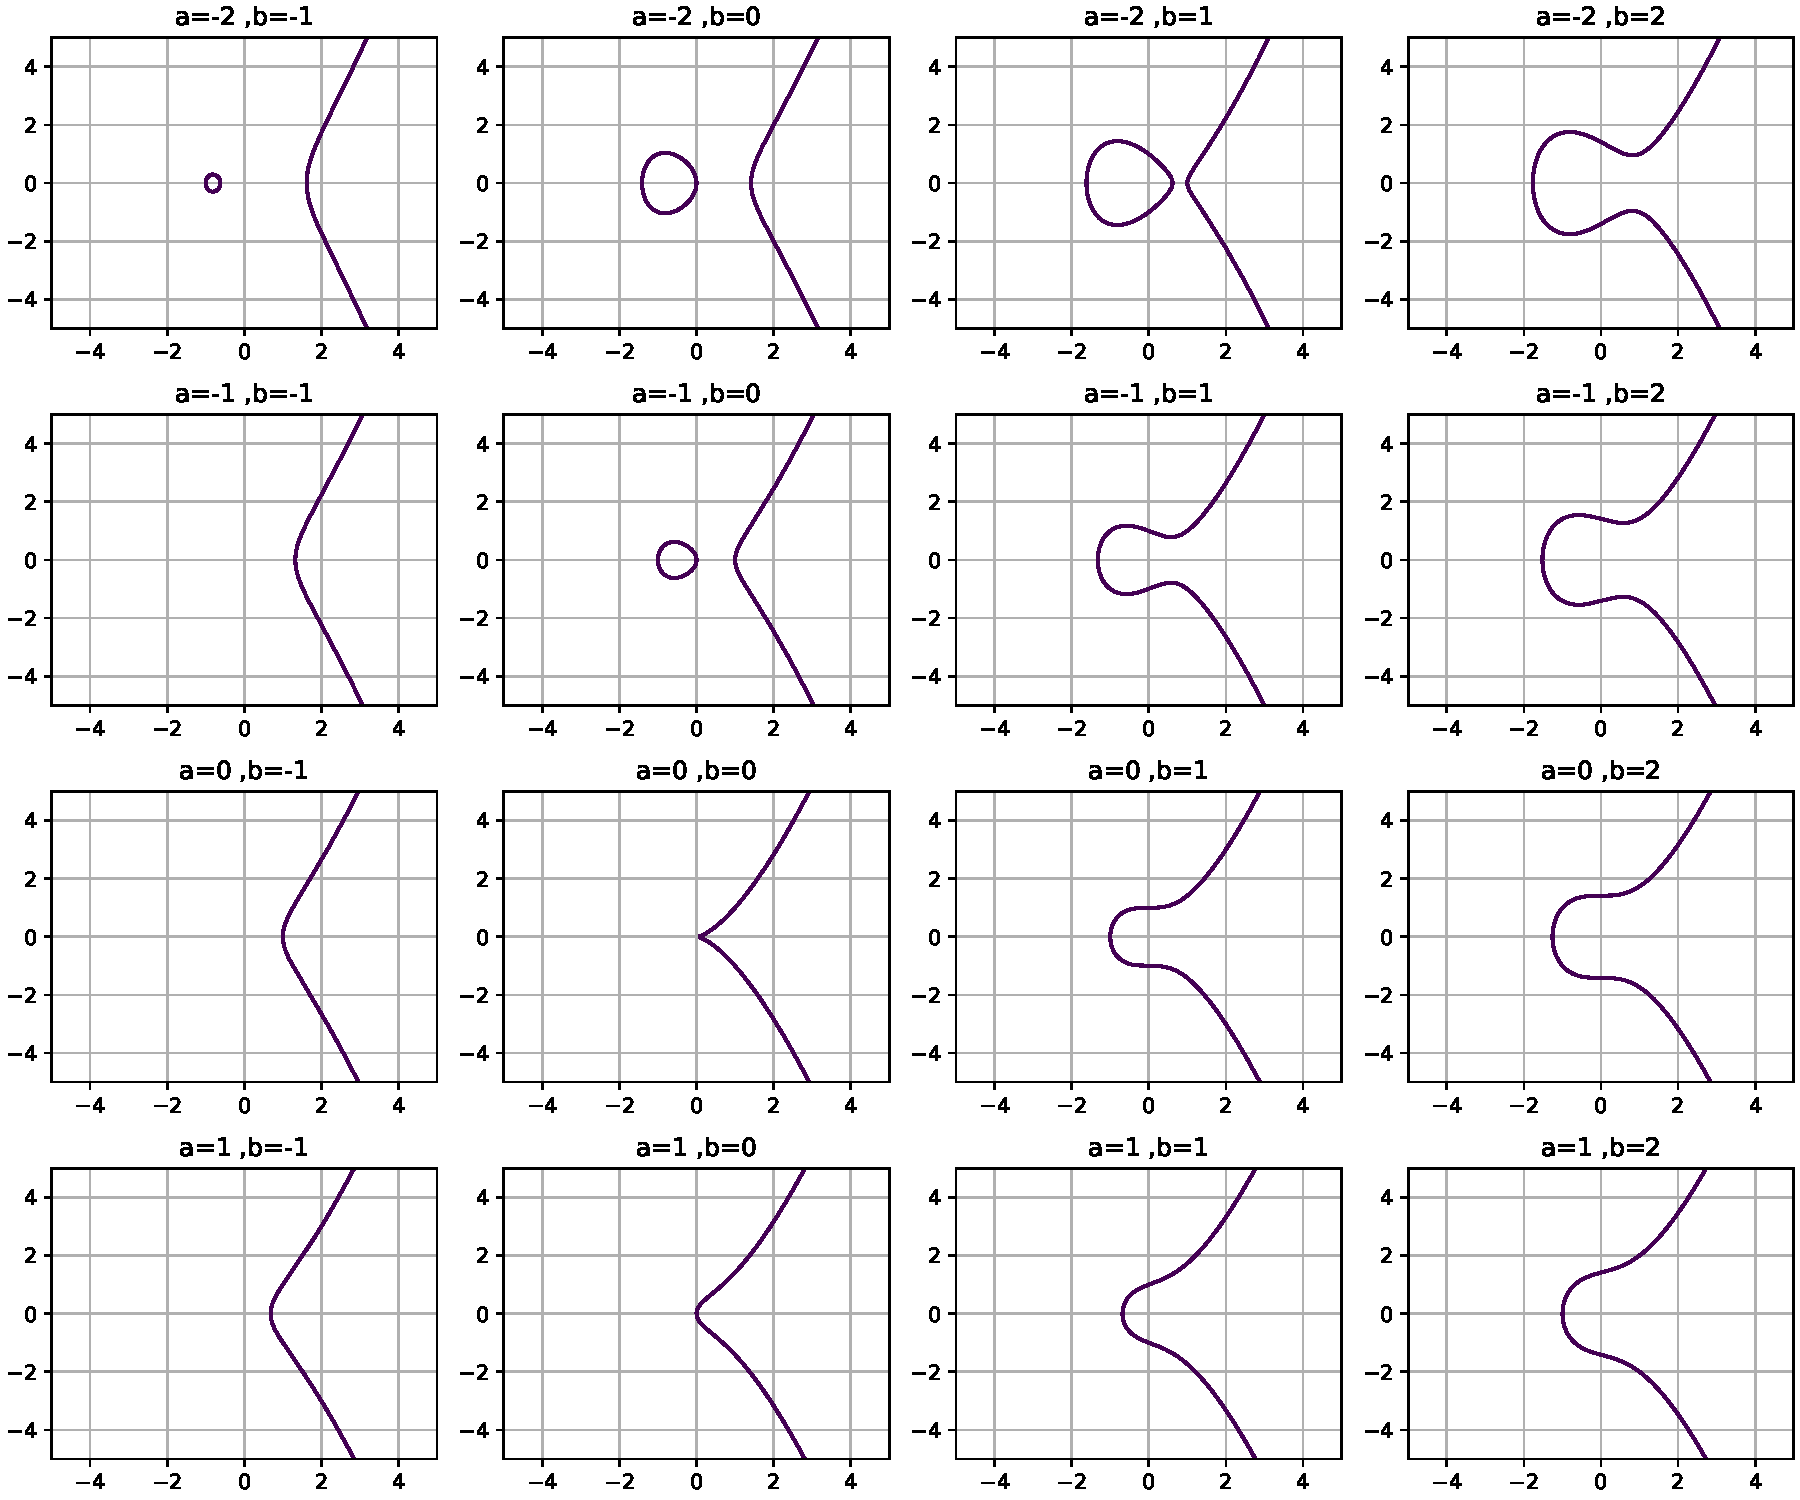
\includegraphics[width=1\linewidth]{./figure/elliptic_curves.pdf}
    \caption{Elliptic curves \cite{childsUniversalComputationQuantum2009} }
\end{figure}


\section{Algorithm}
% \begin{center}
% \begin{minipage}{.9\linewidth}
% algorithm2e
% https://www.overleaf.com/learn/latex/Algorithms#The_algorithm2e_package
\begin{algorithm}[H]
    \SetKwInOut{Input}{input}
    \SetKwInOut{Output}{output}
    \Input{Integer $N$ and parameter $1^t$}
    \Output{A decision as to whether $N$ is prime or composite}
    \BlankLine
    \For{ $i = 1,2, \ldots, t$} {
        $a\leftarrow \qty{1,\dots,N_1}$\;
        \If{$a^{N-1} \neq 1 \mod{N}$}
    {\Return "composite"}
    }
    \Return "prime"
    \caption{Primality testing - first attempt}
    \label{alg:miller_rabin}
\end{algorithm}
% \end{minipage}
% \end{center}

%\part{Computer Science}
% \input{./chapter/complexity.tex}
%% !TEX root = ../notes_template.tex
\chapter{Machine Learning}\label{chp:machine_learning}

\gls{algorithm};
\gls{svm};
\gls{gd};
\glsxtrshort{gd}

% \input{./chapter/algorithms.tex}

%\part{Physics}
%% !TEX root = ../notes_template.tex
\chapter{Quantum Mechanics}\label{chp:quantum_mechanics}

\gls{hamiltonian};
\gls{qft};
\glsxtrshort{qm};
\gls{lagrangian}

% \input{./chapter/quantum_field_theory.tex}

%\begin{appendices}
%% !TEX root = ../notes_template.tex
\chapter{Formulas}

\section{Gaussian distribution}\label{sec:gaussian_distribution}
\begin{definition}[Gaussian distribution]\label{def:gaussian_distribution}
    \myindex{Gaussian distribution}
\end{definition}

\begin{theorem}[Central limit theorem]\label{thm:central_limit_theorem}
\end{theorem}
%\end{appendices}

\backmatter

%%%%%%%%%%%%%%% Reference %%%%%%%%%%%%%%%

\printbibliography[heading=bibintoc]
\printindex

\end{document}

